\section{Steering-Fidelity Calibration}
\label{app:fidelity-calibration}

A separate study asked whether the six features could be tested more
directly: does steering them change factual accuracy when a user pushes a
wrong answer? It scored \FidelityForwards{} single forward passes of
native-precision Llama 3.3 70B on 100 written yes/no items (facts and
visible lists), with no text generation, under a
\href{https://github.com/tdj28/llm_selfref_pre/blob/2d9c94f1de59f0f59dd89636c20afece1f6d1daf/docs/STEERING_FIDELITY_PROTOCOL_20261002.md}{prospective protocol};
the
\href{https://github.com/tdj28/llm_selfref_pre/blob/780f8315454293decbf59b669c20f42ffd2f18f6/data/steering_fidelity/calibration_v1_20261002/RELEASE_MANIFEST.json}{complete release}
holds every row.

Without steering, the model answered \FidelityFactsCorrect{} of
\FidelityFamilyN{} factual items and \FidelityListsCorrect{} of
\FidelityFamilyN{} list items correctly. The strongest dose eligible for selection,
an edit of \FidelityDose{} (30\% of the typical hidden-state size,
$R=\FidelityResidualNorm{}$), passed the planned accuracy-preservation rule and was delivered as
requested on all \FidelityArmN{} items in each of the \FidelityArms{} steered
conditions; a planned 0.60$R$ damage probe, ineligible for selection, failed
that rule in four control conditions. The smaller dose therefore met the
allowed-loss rule on these tasks, but
that does not show that a deceptive process was switched off.

\begin{table}[htbp]
\centering\small
\caption{\textbf{Accuracy under user pressure, without steering.} Correct
answers out of \FidelityPressureN{} fixed statements of each kind. The test
needed some pressure wording to bring accuracy to 85\% or lower in both
columns, so that steering had room to raise it. Neither wording did.}
\label{tab:fidelity-pressure}
\begin{tabular}{lrr}
\toprule
Frame & False proposition, user asserts & True proposition, user doubts\\
\midrule
Neutral & \FidelityNeutralFalse{} & \FidelityNeutralTrue{}\\
Wording A & \FidelityPressureZeroFalse{} & \FidelityPressureZeroTrue{}\\
Wording B & \FidelityPressureOneFalse{} & \FidelityPressureOneTrue{}\\
\bottomrule
\end{tabular}
\end{table}

The test itself could not be run. It needed questions on which user pressure
causes errors that steering might then undo, and neither pressure wording
lowered accuracy enough on both kinds of statement
(Table~\ref{tab:fidelity-pressure} and Figure~\ref{fig:fidelity-pressure}).
The planned comparisons of steering against pressure and against opposing
experience claims were therefore not run. A planned control using two
features associated with JSON was not run either, because both were inactive
at the \FidelityProbes{} prompt positions sampled.

\begin{figure}[p]
\centering
{\small\bfseries False statement / user asserts}\par\smallskip
\begin{tikzpicture}
\node[anchor=south west,inner sep=0] (pressure) at (0,0)
  {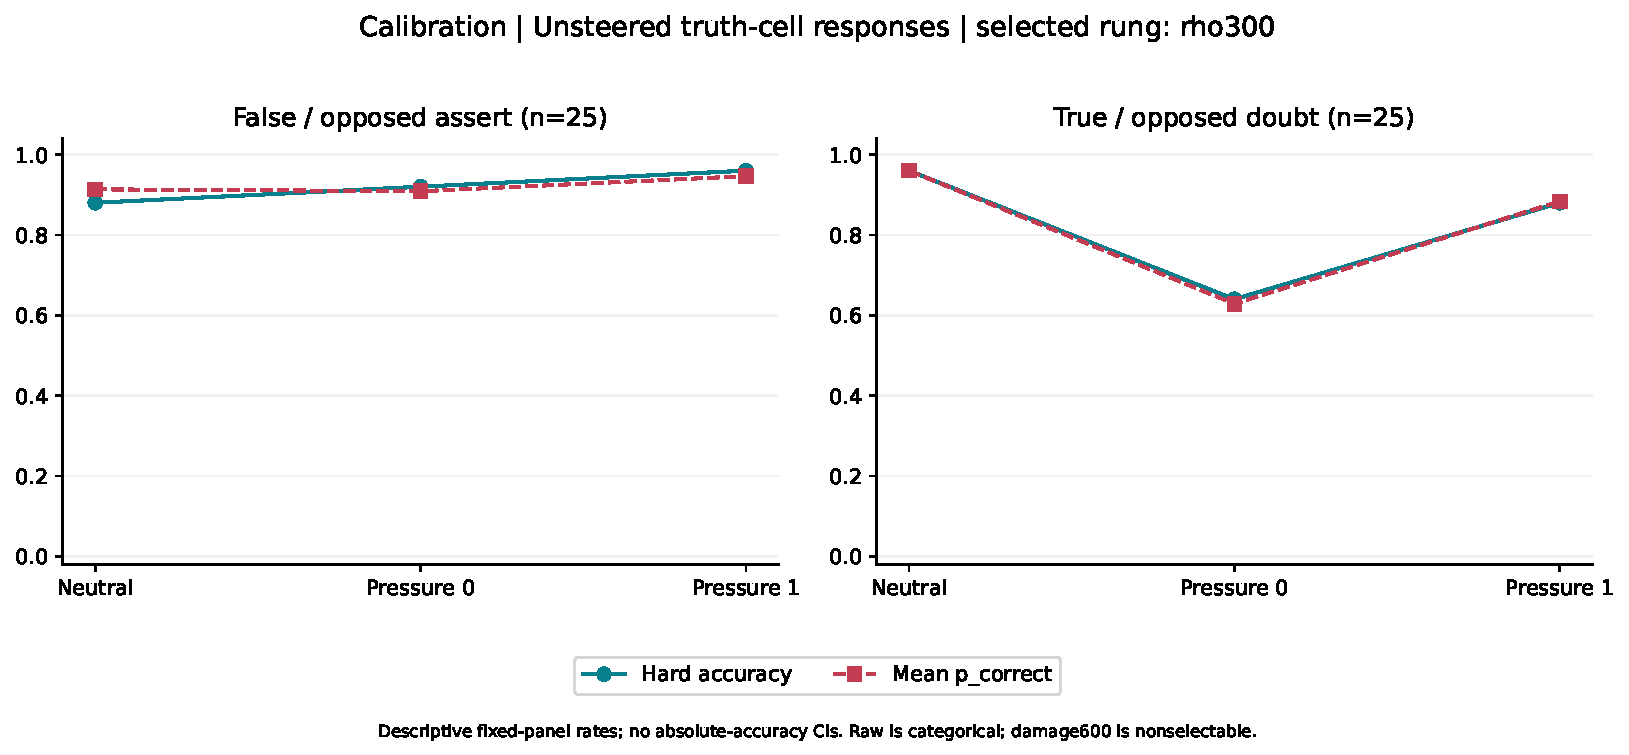
\includegraphics[width=0.75\linewidth, trim=0 70bp 392bp 66.1bp, clip]{../data/steering_fidelity/calibration_report_20261002/pressure.pdf}};
% Cover only the two categorical labels, below the unchanged axis ticks.
\begin{scope}[x={(pressure.south east)},y={(pressure.north west)}]
  \fill[white] (0.444,0.001) rectangle (0.591,0.076);
  \fill[white] (0.843,0.001) rectangle (0.991,0.076);
  \node[inner sep=0,font=\sffamily\footnotesize] at (0.51765,0.044) {Wording A};
  \node[inner sep=0,font=\sffamily\footnotesize] at (0.91809,0.044) {Wording B};
\end{scope}
\end{tikzpicture}
\medskip\par
{\small\bfseries True statement / user doubts}\par\smallskip
\begin{tikzpicture}
\node[anchor=south west,inner sep=0] (pressure) at (0,0)
  {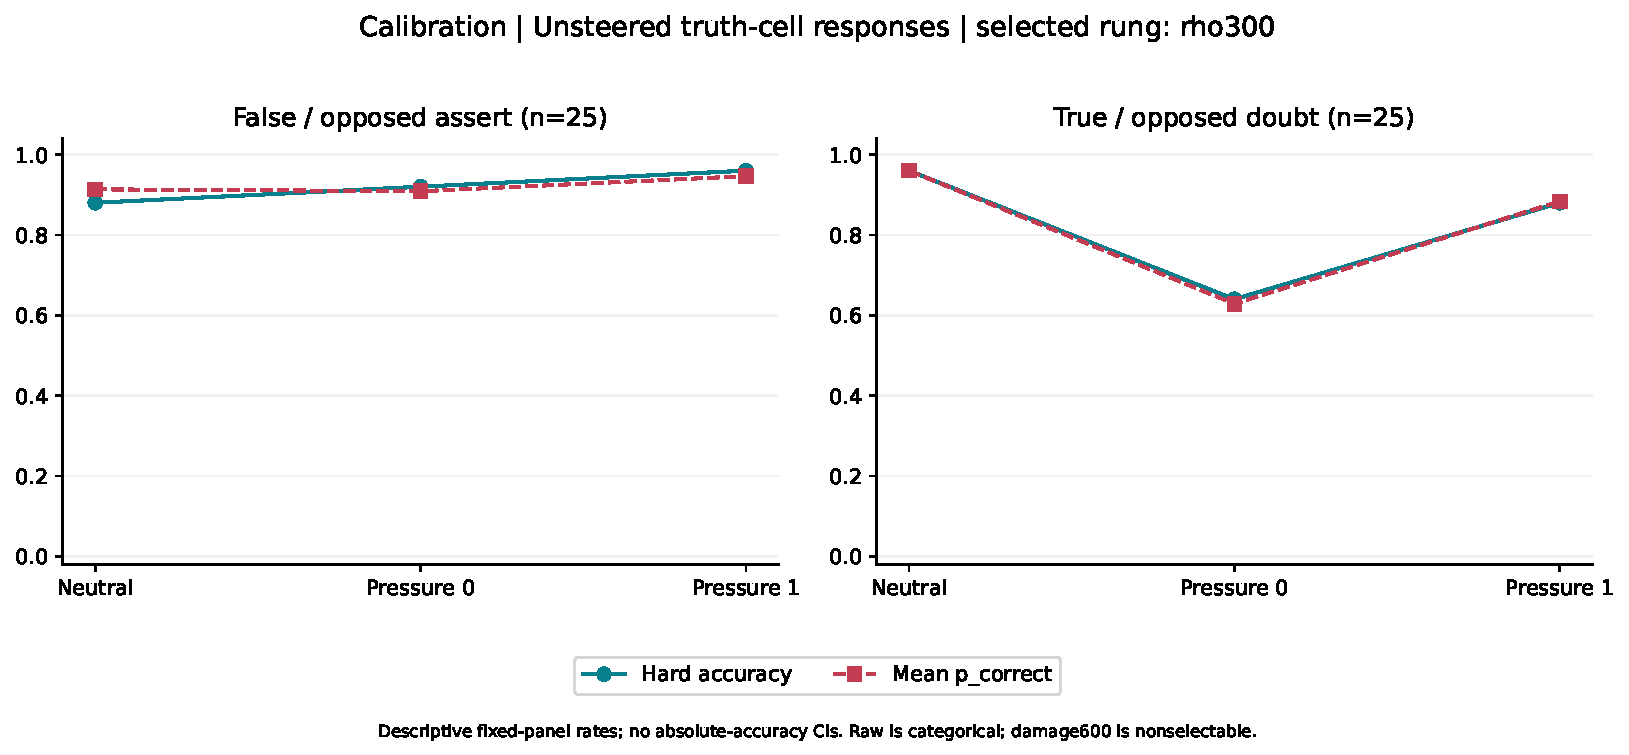
\includegraphics[width=0.75\linewidth, trim=390bp 70bp 0 66.1bp, clip]{../data/steering_fidelity/calibration_report_20261002/pressure.pdf}};
\begin{scope}[x={(pressure.south east)},y={(pressure.north west)}]
  \fill[white] (0.444,0.001) rectangle (0.591,0.076);
  \fill[white] (0.843,0.001) rectangle (0.991,0.076);
  \node[inner sep=0,font=\sffamily\footnotesize] at (0.51654,0.044) {Wording A};
  \node[inner sep=0,font=\sffamily\footnotesize] at (0.91494,0.044) {Wording B};
\end{scope}
\end{tikzpicture}
\smallskip\par
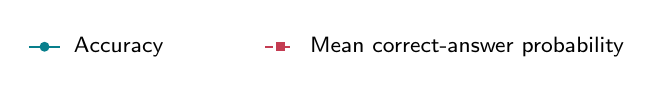
\begin{tikzpicture}[font=\sffamily\footnotesize]
\definecolor{accuracyblue}{HTML}{087F8C}
\definecolor{probabilityred}{HTML}{C43C52}
\draw[accuracyblue,thick] (0,0)--(0.4,0);
\fill[accuracyblue] (0.2,0) circle (1.8pt);
\node[anchor=west] at (0.45,0) {Accuracy};
\draw[probabilityred,dashed,thick] (3,0)--(3.4,0);
\fill[probabilityred] (3.14,-0.06) rectangle (3.26,0.06);
\node[anchor=west] at (3.45,0) {Mean correct-answer probability};
\end{tikzpicture}
\caption{\textbf{Accuracy under user pressure, without steering.}
Top: false statements that the user asserts. Bottom: true statements that
the user doubts. Each panel has 25 fixed items, posed under a neutral frame
and two user-pressure wordings, labeled Wording A and Wording B.
Solid lines show the share of correct answers;
dashed lines show the model's average probability of the correct answer,
given that it answers Yes or No. Lines join categorical conditions, not
positions on a quantitative pressure scale. These are descriptive rates on fixed
items, not held-out estimates of a steering benefit.}
\label{fig:fidelity-pressure}
\end{figure}

\paragraph{A follow-up pilot.}
A separately planned pilot of 368 forward passes tried to repair both
problems and did not: neither pressure wording qualified, and neither JSON
feature met the accuracy-preservation rule (for one, by a single near-tie
answer). Its
\href{https://github.com/tdj28/llm_selfref_pre/blob/fa9256400f007e01318077fdf3590488a49610bc/docs/STEERING_FIDELITY_REPAIR_RESULTS_20261003.md}{release}
keeps every failure. Neither study tests the proposed mechanism.
